\documentclass[1p]{elsarticle_modified}
%\bibliographystyle{elsarticle-num}

%\usepackage[colorlinks]{hyperref}
%\usepackage{abbrmath_seonhwa} %\Abb, \Ascr, \Acal ,\Abf, \Afrak
\usepackage{amsfonts}
\usepackage{amssymb}
\usepackage{amsmath}
\usepackage{amsthm}
\usepackage{scalefnt}
\usepackage{amsbsy}
\usepackage{kotex}
\usepackage{caption}
\usepackage{subfig}
\usepackage{color}
\usepackage{graphicx}
\usepackage{xcolor} %% white, black, red, green, blue, cyan, magenta, yellow
\usepackage{float}
\usepackage{setspace}
\usepackage{hyperref}

\usepackage{tikz}
\usetikzlibrary{arrows}

\usepackage{multirow}
\usepackage{array} % fixed length table
\usepackage{hhline}

%%%%%%%%%%%%%%%%%%%%%
\makeatletter
\renewcommand*\env@matrix[1][\arraystretch]{%
	\edef\arraystretch{#1}%
	\hskip -\arraycolsep
	\let\@ifnextchar\new@ifnextchar
	\array{*\c@MaxMatrixCols c}}
\makeatother %https://tex.stackexchange.com/questions/14071/how-can-i-increase-the-line-spacing-in-a-matrix
%%%%%%%%%%%%%%%

\usepackage[normalem]{ulem}

\newcommand{\msout}[1]{\ifmmode\text{\sout{\ensuremath{#1}}}\else\sout{#1}\fi}
%SOURCE: \msout is \stkout macro in https://tex.stackexchange.com/questions/20609/strikeout-in-math-mode

\newcommand{\cancel}[1]{
	\ifmmode
	{\color{red}\msout{#1}}
	\else
	{\color{red}\sout{#1}}
	\fi
}

\newcommand{\add}[1]{
	{\color{blue}\uwave{#1}}
}

\newcommand{\replace}[2]{
	\ifmmode
	{\color{red}\msout{#1}}{\color{blue}\uwave{#2}}
	\else
	{\color{red}\sout{#1}}{\color{blue}\uwave{#2}}
	\fi
}

\newcommand{\Sol}{\mathcal{S}} %segment
\newcommand{\D}{D} %diagram
\newcommand{\A}{\mathcal{A}} %arc


%%%%%%%%%%%%%%%%%%%%%%%%%%%%%5 test

\def\sl{\operatorname{\textup{SL}}(2,\Cbb)}
\def\psl{\operatorname{\textup{PSL}}(2,\Cbb)}
\def\quan{\mkern 1mu \triangleright \mkern 1mu}

\theoremstyle{definition}
\newtheorem{thm}{Theorem}[section]
\newtheorem{prop}[thm]{Proposition}
\newtheorem{lem}[thm]{Lemma}
\newtheorem{ques}[thm]{Question}
\newtheorem{cor}[thm]{Corollary}
\newtheorem{defn}[thm]{Definition}
\newtheorem{exam}[thm]{Example}
\newtheorem{rmk}[thm]{Remark}
\newtheorem{alg}[thm]{Algorithm}

\newcommand{\I}{\sqrt{-1}}
\begin{document}

%\begin{frontmatter}
%
%\title{Boundary parabolic representations of knots up to 8 crossings}
%
%%% Group authors per affiliation:
%\author{Yunhi Cho} 
%\address{Department of Mathematics, University of Seoul, Seoul, Korea}
%\ead{yhcho@uos.ac.kr}
%
%
%\author{Seonhwa Kim} %\fnref{s_kim}}
%\address{Center for Geometry and Physics, Institute for Basic Science, Pohang, 37673, Korea}
%\ead{ryeona17@ibs.re.kr}
%
%\author{Hyuk Kim}
%\address{Department of Mathematical Sciences, Seoul National University, Seoul 08826, Korea}
%\ead{hyukkim@snu.ac.kr}
%
%\author{Seokbeom Yoon}
%\address{Department of Mathematical Sciences, Seoul National University, Seoul, 08826,  Korea}
%\ead{sbyoon15@snu.ac.kr}
%
%\begin{abstract}
%We find all boundary parabolic representation of knots up to 8 crossings.
%
%\end{abstract}
%\begin{keyword}
%    \MSC[2010] 57M25 
%\end{keyword}
%
%\end{frontmatter}

%\linenumbers
%\tableofcontents
%
\newcommand\colored[1]{\textcolor{white}{\rule[-0.35ex]{0.8em}{1.4ex}}\kern-0.8em\color{red} #1}%
%\newcommand\colored[1]{\textcolor{white}{ #1}\kern-2.17ex	\textcolor{white}{ #1}\kern-1.81ex	\textcolor{white}{ #1}\kern-2.15ex\color{red}#1	}

{\Large $\underline{12a_{0192}~(K12a_{0192})}$}

\setlength{\tabcolsep}{10pt}
\renewcommand{\arraystretch}{1.6}
\vspace{1cm}\begin{tabular}{m{100pt}>{\centering\arraybackslash}m{274pt}}
\multirow{5}{120pt}{
	\centering
	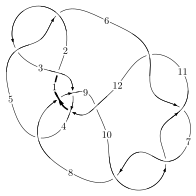
\includegraphics[width=112pt]{../../../GIT/diagram.site/Diagrams/png/993_12a_0192.png}\\
\ \ \ A knot diagram\footnotemark}&
\allowdisplaybreaks
\textbf{Linearized knot diagam} \\
\cline{2-2}
 &
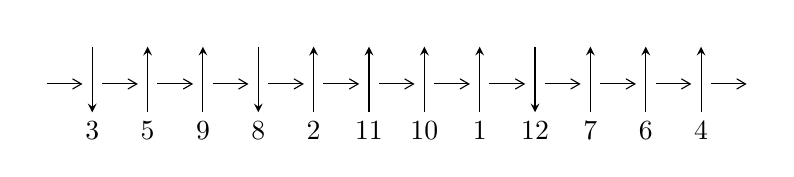
\begin{tikzpicture}[x=20pt, y=17pt]
	% nodes
	\node (C0) at (0, 0) {};
	\node (C1) at (1, 0) {};
	\node (C1U) at (1, +1) {};
	\node (C1D) at (1, -1) {3};

	\node (C2) at (2, 0) {};
	\node (C2U) at (2, +1) {};
	\node (C2D) at (2, -1) {5};

	\node (C3) at (3, 0) {};
	\node (C3U) at (3, +1) {};
	\node (C3D) at (3, -1) {9};

	\node (C4) at (4, 0) {};
	\node (C4U) at (4, +1) {};
	\node (C4D) at (4, -1) {8};

	\node (C5) at (5, 0) {};
	\node (C5U) at (5, +1) {};
	\node (C5D) at (5, -1) {2};

	\node (C6) at (6, 0) {};
	\node (C6U) at (6, +1) {};
	\node (C6D) at (6, -1) {11};

	\node (C7) at (7, 0) {};
	\node (C7U) at (7, +1) {};
	\node (C7D) at (7, -1) {10};

	\node (C8) at (8, 0) {};
	\node (C8U) at (8, +1) {};
	\node (C8D) at (8, -1) {1};

	\node (C9) at (9, 0) {};
	\node (C9U) at (9, +1) {};
	\node (C9D) at (9, -1) {12};

	\node (C10) at (10, 0) {};
	\node (C10U) at (10, +1) {};
	\node (C10D) at (10, -1) {7};

	\node (C11) at (11, 0) {};
	\node (C11U) at (11, +1) {};
	\node (C11D) at (11, -1) {6};

	\node (C12) at (12, 0) {};
	\node (C12U) at (12, +1) {};
	\node (C12D) at (12, -1) {4};
	\node (C13) at (13, 0) {};

	% arrows
	\draw[->,>={angle 60}]
	(C0) edge (C1) (C1) edge (C2) (C2) edge (C3) (C3) edge (C4) (C4) edge (C5) (C5) edge (C6) (C6) edge (C7) (C7) edge (C8) (C8) edge (C9) (C9) edge (C10) (C10) edge (C11) (C11) edge (C12) (C12) edge (C13) ;	\draw[->,>=stealth]
	(C1U) edge (C1D) (C2D) edge (C2U) (C3D) edge (C3U) (C4U) edge (C4D) (C5D) edge (C5U) (C6D) edge (C6U) (C7D) edge (C7U) (C8D) edge (C8U) (C9U) edge (C9D) (C10D) edge (C10U) (C11D) edge (C11U) (C12D) edge (C12U) ;
	\end{tikzpicture} \\
\hhline{~~} \\& 
\textbf{Solving Sequence} \\ \cline{2-2} 
 &
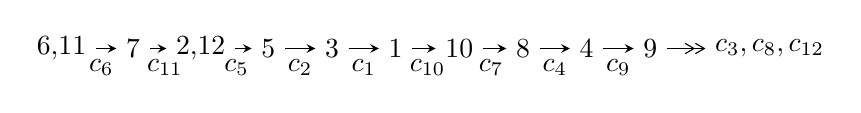
\begin{tikzpicture}[x=23pt, y=7pt]
	% node
	\node (A0) at (-1/8, 0) {6,11};
	\node (A1) at (1, 0) {7};
	\node (A2) at (33/16, 0) {2,12};
	\node (A3) at (25/8, 0) {5};
	\node (A4) at (33/8, 0) {3};
	\node (A5) at (41/8, 0) {1};
	\node (A6) at (49/8, 0) {10};
	\node (A7) at (57/8, 0) {8};
	\node (A8) at (65/8, 0) {4};
	\node (A9) at (73/8, 0) {9};
	\node (C1) at (1/2, -1) {$c_{6}$};
	\node (C2) at (3/2, -1) {$c_{11}$};
	\node (C3) at (21/8, -1) {$c_{5}$};
	\node (C4) at (29/8, -1) {$c_{2}$};
	\node (C5) at (37/8, -1) {$c_{1}$};
	\node (C6) at (45/8, -1) {$c_{10}$};
	\node (C7) at (53/8, -1) {$c_{7}$};
	\node (C8) at (61/8, -1) {$c_{4}$};
	\node (C9) at (69/8, -1) {$c_{9}$};
	\node (A10) at (11, 0) {$c_{3},c_{8},c_{12}$};

	% edge
	\draw[->,>=stealth]	
	(A0) edge (A1) (A1) edge (A2) (A2) edge (A3) (A3) edge (A4) (A4) edge (A5) (A5) edge (A6) (A6) edge (A7) (A7) edge (A8) (A8) edge (A9) ;
	\draw[->>,>={angle 60}]	
	(A9) edge (A10);
\end{tikzpicture} \\ 

\end{tabular} \\

\footnotetext{
The image of knot diagram is generated by the software ``\textbf{Draw programme}" developed by Andrew Bartholomew(\url{http://www.layer8.co.uk/maths/draw/index.htm\#Running-draw}), where we modified some parts for our purpose(\url{https://github.com/CATsTAILs/LinksPainter}).
}\phantom \\ \newline 
\centering \textbf{Ideals for irreducible components\footnotemark of $X_{\text{par}}$} 
 
\begin{align*}
I^u_{1}&=\langle 
-7.37926\times10^{55} u^{88}+9.52831\times10^{57} u^{87}+\cdots+4.66485\times10^{58} b+1.81070\times10^{58},\\
\phantom{I^u_{1}}&\phantom{= \langle  }3.57832\times10^{57} u^{88}-1.08873\times10^{58} u^{87}+\cdots+4.66485\times10^{58} a-5.48631\times10^{58},\;u^{89}+u^{88}+\cdots+5 u-1\rangle \\
\\
\end{align*}
\raggedright * 1 irreducible components of $\dim_{\mathbb{C}}=0$, with total 89 representations.\\
\footnotetext{All coefficients of polynomials are rational numbers. But the coefficients are sometimes approximated in decimal forms when there is not enough margin.}
\newpage
\renewcommand{\arraystretch}{1}
\centering \section*{I. $I^u_{1}= \langle -7.38\times10^{55} u^{88}+9.53\times10^{57} u^{87}+\cdots+4.66\times10^{58} b+1.81\times10^{58},\;3.58\times10^{57} u^{88}-1.09\times10^{58} u^{87}+\cdots+4.66\times10^{58} a-5.49\times10^{58},\;u^{89}+u^{88}+\cdots+5 u-1 \rangle$}
\flushleft \textbf{(i) Arc colorings}\\
\begin{tabular}{m{7pt} m{180pt} m{7pt} m{180pt} }
\flushright $a_{6}=$&$\begin{pmatrix}1\\0\end{pmatrix}$ \\
\flushright $a_{11}=$&$\begin{pmatrix}0\\u\end{pmatrix}$ \\
\flushright $a_{7}=$&$\begin{pmatrix}1\\- u^2\end{pmatrix}$ \\
\flushright $a_{2}=$&$\begin{pmatrix}-0.0767082 u^{88}+0.233391 u^{87}+\cdots+2.20793 u+1.17610\\0.00158188 u^{88}-0.204257 u^{87}+\cdots+4.22139 u-0.388158\end{pmatrix}$ \\
\flushright $a_{12}=$&$\begin{pmatrix}u\\u\end{pmatrix}$ \\
\flushright $a_{5}=$&$\begin{pmatrix}-0.0700335 u^{88}+0.955530 u^{87}+\cdots+6.31059 u-0.164482\\0.000780172 u^{88}-0.187319 u^{87}+\cdots+3.98539 u-1.30273\end{pmatrix}$ \\
\flushright $a_{3}=$&$\begin{pmatrix}-0.0962203 u^{88}+0.711962 u^{87}+\cdots+9.34457 u-1.31376\\-0.0299682 u^{88}-0.276739 u^{87}+\cdots+3.53290 u-1.29576\end{pmatrix}$ \\
\flushright $a_{1}=$&$\begin{pmatrix}-0.0570863 u^{88}+0.575773 u^{87}+\cdots+0.462546 u-1.20248\\0.780343 u^{88}+0.632859 u^{87}+\cdots+3.82209 u-0.837430\end{pmatrix}$ \\
\flushright $a_{10}=$&$\begin{pmatrix}- u\\u^3+u\end{pmatrix}$ \\
\flushright $a_{8}=$&$\begin{pmatrix}u^2+1\\- u^4-2 u^2\end{pmatrix}$ \\
\flushright $a_{4}=$&$\begin{pmatrix}-0.368118 u^{88}-0.575274 u^{87}+\cdots+5.72052 u-0.661402\\-0.0758137 u^{88}-0.403033 u^{87}+\cdots-2.02265 u+0.00119394\end{pmatrix}$ \\
\flushright $a_{9}=$&$\begin{pmatrix}u^5+2 u^3- u\\u^5+3 u^3+u\end{pmatrix}$\\&\end{tabular}
\flushleft \textbf{(ii) Obstruction class $= -1$}\\~\\
\flushleft \textbf{(iii) Cusp Shapes $= -3.67855 u^{88}-1.96081 u^{87}+\cdots-19.9102 u+7.42306$}\\~\\
\newpage\renewcommand{\arraystretch}{1}
\flushleft \textbf{(iv) u-Polynomials at the component}\newline \\
\begin{tabular}{m{50pt}|m{274pt}}
Crossings & \hspace{64pt}u-Polynomials at each crossing \\
\hline $$\begin{aligned}c_{1}\end{aligned}$$&$\begin{aligned}
&u^{89}+35 u^{88}+\cdots+9 u-1
\end{aligned}$\\
\hline $$\begin{aligned}c_{2},c_{5}\end{aligned}$$&$\begin{aligned}
&u^{89}+u^{88}+\cdots+9 u-1
\end{aligned}$\\
\hline $$\begin{aligned}c_{3}\end{aligned}$$&$\begin{aligned}
&u^{89}+u^{88}+\cdots-1279 u-421
\end{aligned}$\\
\hline $$\begin{aligned}c_{4}\end{aligned}$$&$\begin{aligned}
&u^{89}+3 u^{88}+\cdots+1113 u-503
\end{aligned}$\\
\hline $$\begin{aligned}c_{6},c_{7},c_{10}\\c_{11}\end{aligned}$$&$\begin{aligned}
&u^{89}+u^{88}+\cdots+5 u-1
\end{aligned}$\\
\hline $$\begin{aligned}c_{8}\end{aligned}$$&$\begin{aligned}
&u^{89}-5 u^{88}+\cdots+u-1
\end{aligned}$\\
\hline $$\begin{aligned}c_{9}\end{aligned}$$&$\begin{aligned}
&u^{89}-19 u^{88}+\cdots+158017 u-14627
\end{aligned}$\\
\hline $$\begin{aligned}c_{12}\end{aligned}$$&$\begin{aligned}
&u^{89}+9 u^{88}+\cdots- u-1
\end{aligned}$\\
\hline
\end{tabular}\\~\\
\newpage\renewcommand{\arraystretch}{1}
\flushleft \textbf{(v) Riley Polynomials at the component}\newline \\
\begin{tabular}{m{50pt}|m{274pt}}
Crossings & \hspace{64pt}Riley Polynomials at each crossing \\
\hline $$\begin{aligned}c_{1}\end{aligned}$$&$\begin{aligned}
&y^{89}+39 y^{88}+\cdots-651 y-1
\end{aligned}$\\
\hline $$\begin{aligned}c_{2},c_{5}\end{aligned}$$&$\begin{aligned}
&y^{89}+35 y^{88}+\cdots+9 y-1
\end{aligned}$\\
\hline $$\begin{aligned}c_{3}\end{aligned}$$&$\begin{aligned}
&y^{89}-109 y^{88}+\cdots+13004525 y-177241
\end{aligned}$\\
\hline $$\begin{aligned}c_{4}\end{aligned}$$&$\begin{aligned}
&y^{89}-81 y^{88}+\cdots-6843435 y-253009
\end{aligned}$\\
\hline $$\begin{aligned}c_{6},c_{7},c_{10}\\c_{11}\end{aligned}$$&$\begin{aligned}
&y^{89}+99 y^{88}+\cdots+5 y-1
\end{aligned}$\\
\hline $$\begin{aligned}c_{8}\end{aligned}$$&$\begin{aligned}
&y^{89}-9 y^{88}+\cdots+5 y-1
\end{aligned}$\\
\hline $$\begin{aligned}c_{9}\end{aligned}$$&$\begin{aligned}
&y^{89}+27 y^{88}+\cdots-8680509275 y-213949129
\end{aligned}$\\
\hline $$\begin{aligned}c_{12}\end{aligned}$$&$\begin{aligned}
&y^{89}-5 y^{88}+\cdots+9 y-1
\end{aligned}$\\
\hline
\end{tabular}\\~\\
\newpage\flushleft \textbf{(vi) Complex Volumes and Cusp Shapes}
$$\begin{array}{c|c|c}  
\text{Solutions to }I^u_{1}& \I (\text{vol} + \sqrt{-1}CS) & \text{Cusp shape}\\
 \hline 
\begin{aligned}
u &= \phantom{-}0.629172 + 0.711509 I \\
a &= \phantom{-}1.44311 - 1.26130 I \\
b &= -0.589163 - 0.910663 I\end{aligned}
 & \phantom{-}1.38416 + 5.67170 I & \phantom{-0.000000 } 0 \\ \hline\begin{aligned}
u &= \phantom{-}0.629172 - 0.711509 I \\
a &= \phantom{-}1.44311 + 1.26130 I \\
b &= -0.589163 + 0.910663 I\end{aligned}
 & \phantom{-}1.38416 - 5.67170 I & \phantom{-0.000000 } 0 \\ \hline\begin{aligned}
u &= \phantom{-}0.222782 + 0.904277 I \\
a &= -0.111171 + 0.701310 I \\
b &= -0.556330 + 0.569146 I\end{aligned}
 & -0.83522 + 2.21982 I & \phantom{-0.000000 } 0 \\ \hline\begin{aligned}
u &= \phantom{-}0.222782 - 0.904277 I \\
a &= -0.111171 - 0.701310 I \\
b &= -0.556330 - 0.569146 I\end{aligned}
 & -0.83522 - 2.21982 I & \phantom{-0.000000 } 0 \\ \hline\begin{aligned}
u &= \phantom{-}0.652354 + 0.618933 I \\
a &= \phantom{-}0.016156 - 0.206879 I \\
b &= -0.568168 + 0.764733 I\end{aligned}
 & \phantom{-}1.84881 + 1.03677 I & \phantom{-0.000000 } 0 \\ \hline\begin{aligned}
u &= \phantom{-}0.652354 - 0.618933 I \\
a &= \phantom{-}0.016156 + 0.206879 I \\
b &= -0.568168 - 0.764733 I\end{aligned}
 & \phantom{-}1.84881 - 1.03677 I & \phantom{-0.000000 } 0 \\ \hline\begin{aligned}
u &= -0.587821 + 0.668605 I \\
a &= \phantom{-}1.84371 + 1.57426 I \\
b &= -0.689784 + 1.112970 I\end{aligned}
 & \phantom{-}1.6805 - 14.3965 I & \phantom{-0.000000 } 0 \\ \hline\begin{aligned}
u &= -0.587821 - 0.668605 I \\
a &= \phantom{-}1.84371 - 1.57426 I \\
b &= -0.689784 - 1.112970 I\end{aligned}
 & \phantom{-}1.6805 + 14.3965 I & \phantom{-0.000000 } 0 \\ \hline\begin{aligned}
u &= -0.576040 + 0.637409 I \\
a &= -0.180456 + 0.891479 I \\
b &= -0.912731 - 0.519289 I\end{aligned}
 & \phantom{-}3.49714 - 8.50503 I & \phantom{-0.000000 } 0 \\ \hline\begin{aligned}
u &= -0.576040 - 0.637409 I \\
a &= -0.180456 - 0.891479 I \\
b &= -0.912731 + 0.519289 I\end{aligned}
 & \phantom{-}3.49714 + 8.50503 I & \phantom{-0.000000 } 0\\
 \hline 
 \end{array}$$\newpage$$\begin{array}{c|c|c}  
\text{Solutions to }I^u_{1}& \I (\text{vol} + \sqrt{-1}CS) & \text{Cusp shape}\\
 \hline 
\begin{aligned}
u &= -0.186133 + 0.807246 I \\
a &= \phantom{-}1.17307 + 2.02621 I \\
b &= -0.110685 + 1.090650 I\end{aligned}
 & -5.27581 + 0.77625 I & \phantom{-0.000000 } 0 \\ \hline\begin{aligned}
u &= -0.186133 - 0.807246 I \\
a &= \phantom{-}1.17307 - 2.02621 I \\
b &= -0.110685 - 1.090650 I\end{aligned}
 & -5.27581 - 0.77625 I & \phantom{-0.000000 } 0 \\ \hline\begin{aligned}
u &= \phantom{-}0.187001 + 1.165500 I \\
a &= \phantom{-}0.45304 - 1.37786 I \\
b &= -0.617348 - 0.979446 I\end{aligned}
 & -1.97335 + 7.02283 I & \phantom{-0.000000 } 0 \\ \hline\begin{aligned}
u &= \phantom{-}0.187001 - 1.165500 I \\
a &= \phantom{-}0.45304 + 1.37786 I \\
b &= -0.617348 + 0.979446 I\end{aligned}
 & -1.97335 - 7.02283 I & \phantom{-0.000000 } 0 \\ \hline\begin{aligned}
u &= -0.483117 + 0.643227 I \\
a &= -1.27197 - 1.41185 I \\
b &= \phantom{-}0.055573 - 1.266110 I\end{aligned}
 & -3.30433 - 6.34543 I & \phantom{-0.000000 -}0. + 9.41566 I \\ \hline\begin{aligned}
u &= -0.483117 - 0.643227 I \\
a &= -1.27197 + 1.41185 I \\
b &= \phantom{-}0.055573 + 1.266110 I\end{aligned}
 & -3.30433 + 6.34543 I & \phantom{-0.000000 } 0. - 9.41566 I \\ \hline\begin{aligned}
u &= \phantom{-}0.735954 + 0.310708 I \\
a &= \phantom{-}1.072010 - 0.285219 I \\
b &= -0.596779 - 0.860932 I\end{aligned}
 & \phantom{-}2.75551 + 3.59145 I & \phantom{-}16.9119 - 7.8798 I \\ \hline\begin{aligned}
u &= \phantom{-}0.735954 - 0.310708 I \\
a &= \phantom{-}1.072010 + 0.285219 I \\
b &= -0.596779 + 0.860932 I\end{aligned}
 & \phantom{-}2.75551 - 3.59145 I & \phantom{-}16.9119 + 7.8798 I \\ \hline\begin{aligned}
u &= -0.128379 + 1.218880 I \\
a &= \phantom{-}0.048603 - 1.126680 I \\
b &= -0.654242 - 1.028240 I\end{aligned}
 & -1.89864 + 7.13164 I & \phantom{-0.000000 } 0 \\ \hline\begin{aligned}
u &= -0.128379 - 1.218880 I \\
a &= \phantom{-}0.048603 + 1.126680 I \\
b &= -0.654242 + 1.028240 I\end{aligned}
 & -1.89864 - 7.13164 I & \phantom{-0.000000 } 0\\
 \hline 
 \end{array}$$\newpage$$\begin{array}{c|c|c}  
\text{Solutions to }I^u_{1}& \I (\text{vol} + \sqrt{-1}CS) & \text{Cusp shape}\\
 \hline 
\begin{aligned}
u &= \phantom{-}0.302285 + 0.698873 I \\
a &= \phantom{-}0.372084 + 1.059710 I \\
b &= -0.097148 + 0.520009 I\end{aligned}
 & -0.88546 + 2.04291 I & \phantom{-}2.01521 - 6.41546 I \\ \hline\begin{aligned}
u &= \phantom{-}0.302285 - 0.698873 I \\
a &= \phantom{-}0.372084 - 1.059710 I \\
b &= -0.097148 - 0.520009 I\end{aligned}
 & -0.88546 - 2.04291 I & \phantom{-}2.01521 + 6.41546 I \\ \hline\begin{aligned}
u &= \phantom{-}0.729548 + 0.201616 I \\
a &= \phantom{-}0.787909 + 0.143124 I \\
b &= -0.594451 + 0.821113 I\end{aligned}
 & \phantom{-}2.87995 - 1.13132 I & \phantom{-}17.8044 + 0. I\phantom{ +0.000000I} \\ \hline\begin{aligned}
u &= \phantom{-}0.729548 - 0.201616 I \\
a &= \phantom{-}0.787909 - 0.143124 I \\
b &= -0.594451 - 0.821113 I\end{aligned}
 & \phantom{-}2.87995 + 1.13132 I & \phantom{-}17.8044 + 0. I\phantom{ +0.000000I} \\ \hline\begin{aligned}
u &= -0.487284 + 0.556003 I \\
a &= -2.04497 - 1.51099 I \\
b &= \phantom{-}0.721154 - 1.156170 I\end{aligned}
 & \phantom{-}1.32467 - 6.17318 I & \phantom{-}8.6449 + 12.1067 I \\ \hline\begin{aligned}
u &= -0.487284 - 0.556003 I \\
a &= -2.04497 + 1.51099 I \\
b &= \phantom{-}0.721154 + 1.156170 I\end{aligned}
 & \phantom{-}1.32467 + 6.17318 I & \phantom{-}8.6449 - 12.1067 I \\ \hline\begin{aligned}
u &= -0.672888 + 0.280476 I \\
a &= \phantom{-}0.789738 - 0.042118 I \\
b &= -0.684732 - 1.084880 I\end{aligned}
 & \phantom{-}2.83010 + 10.15130 I & \phantom{-}7.61075 - 5.74179 I \\ \hline\begin{aligned}
u &= -0.672888 - 0.280476 I \\
a &= \phantom{-}0.789738 + 0.042118 I \\
b &= -0.684732 + 1.084880 I\end{aligned}
 & \phantom{-}2.83010 - 10.15130 I & \phantom{-}7.61075 + 5.74179 I \\ \hline\begin{aligned}
u &= -0.639069 + 0.312530 I \\
a &= \phantom{-}1.053290 + 0.122104 I \\
b &= -0.869417 + 0.551430 I\end{aligned}
 & \phantom{-}4.45557 + 4.38854 I & \phantom{-}10.08298 - 1.27597 I \\ \hline\begin{aligned}
u &= -0.639069 - 0.312530 I \\
a &= \phantom{-}1.053290 - 0.122104 I \\
b &= -0.869417 - 0.551430 I\end{aligned}
 & \phantom{-}4.45557 - 4.38854 I & \phantom{-}10.08298 + 1.27597 I\\
 \hline 
 \end{array}$$\newpage$$\begin{array}{c|c|c}  
\text{Solutions to }I^u_{1}& \I (\text{vol} + \sqrt{-1}CS) & \text{Cusp shape}\\
 \hline 
\begin{aligned}
u &= -0.500387 + 0.501574 I \\
a &= -1.042820 - 0.811706 I \\
b &= \phantom{-}0.978738 - 0.544688 I\end{aligned}
 & \phantom{-}3.39905 - 3.48992 I & \phantom{-}14.4983 + 7.8374 I \\ \hline\begin{aligned}
u &= -0.500387 - 0.501574 I \\
a &= -1.042820 + 0.811706 I \\
b &= \phantom{-}0.978738 + 0.544688 I\end{aligned}
 & \phantom{-}3.39905 + 3.48992 I & \phantom{-}14.4983 - 7.8374 I \\ \hline\begin{aligned}
u &= \phantom{-}0.474265 + 0.491419 I \\
a &= \phantom{-}0.465564 + 0.028509 I \\
b &= \phantom{-}0.173591 + 0.109004 I\end{aligned}
 & \phantom{-}0.68170 + 1.66226 I & \phantom{-}3.48924 - 4.60078 I \\ \hline\begin{aligned}
u &= \phantom{-}0.474265 - 0.491419 I \\
a &= \phantom{-}0.465564 - 0.028509 I \\
b &= \phantom{-}0.173591 - 0.109004 I\end{aligned}
 & \phantom{-}0.68170 - 1.66226 I & \phantom{-}3.48924 + 4.60078 I \\ \hline\begin{aligned}
u &= \phantom{-}0.434724 + 0.524138 I \\
a &= -5.16293 + 0.82804 I \\
b &= \phantom{-}0.537717 + 0.883432 I\end{aligned}
 & \phantom{-}0.38729 + 3.69638 I & -13.5626 + 18.8380 I \\ \hline\begin{aligned}
u &= \phantom{-}0.434724 - 0.524138 I \\
a &= -5.16293 - 0.82804 I \\
b &= \phantom{-}0.537717 - 0.883432 I\end{aligned}
 & \phantom{-}0.38729 - 3.69638 I & -13.5626 - 18.8380 I \\ \hline\begin{aligned}
u &= -0.499673 + 0.459395 I \\
a &= -0.080168 - 1.151680 I \\
b &= \phantom{-}0.969659 + 0.422445 I\end{aligned}
 & \phantom{-}3.52293 - 0.01044 I & \phantom{-}15.3738 + 0.9083 I \\ \hline\begin{aligned}
u &= -0.499673 - 0.459395 I \\
a &= -0.080168 + 1.151680 I \\
b &= \phantom{-}0.969659 - 0.422445 I\end{aligned}
 & \phantom{-}3.52293 + 0.01044 I & \phantom{-}15.3738 - 0.9083 I \\ \hline\begin{aligned}
u &= -0.103485 + 1.347580 I \\
a &= \phantom{-}0.273259 + 0.747966 I \\
b &= -0.786906 + 0.627797 I\end{aligned}
 & -0.67403 + 1.69091 I & \phantom{-0.000000 } 0 \\ \hline\begin{aligned}
u &= -0.103485 - 1.347580 I \\
a &= \phantom{-}0.273259 - 0.747966 I \\
b &= -0.786906 - 0.627797 I\end{aligned}
 & -0.67403 - 1.69091 I & \phantom{-0.000000 } 0\\
 \hline 
 \end{array}$$\newpage$$\begin{array}{c|c|c}  
\text{Solutions to }I^u_{1}& \I (\text{vol} + \sqrt{-1}CS) & \text{Cusp shape}\\
 \hline 
\begin{aligned}
u &= \phantom{-}0.431180 + 0.470567 I \\
a &= -1.96595 + 3.06518 I \\
b &= \phantom{-}0.535306 - 0.833683 I\end{aligned}
 & \phantom{-}0.550681 - 0.619676 I & -20.5386 + 0.0092 I \\ \hline\begin{aligned}
u &= \phantom{-}0.431180 - 0.470567 I \\
a &= -1.96595 - 3.06518 I \\
b &= \phantom{-}0.535306 + 0.833683 I\end{aligned}
 & \phantom{-}0.550681 + 0.619676 I & -20.5386 - 0.0092 I \\ \hline\begin{aligned}
u &= \phantom{-}0.295375 + 0.540642 I \\
a &= \phantom{-}2.09399 - 3.18145 I \\
b &= \phantom{-}0.406553 - 0.839840 I\end{aligned}
 & -0.370699 - 0.487288 I & \phantom{-}9.82844 + 2.22925 I \\ \hline\begin{aligned}
u &= \phantom{-}0.295375 - 0.540642 I \\
a &= \phantom{-}2.09399 + 3.18145 I \\
b &= \phantom{-}0.406553 + 0.839840 I\end{aligned}
 & -0.370699 + 0.487288 I & \phantom{-}9.82844 - 2.22925 I \\ \hline\begin{aligned}
u &= -0.473391 + 0.392852 I \\
a &= -0.181126 - 0.558731 I \\
b &= \phantom{-}0.749485 + 1.073430 I\end{aligned}
 & \phantom{-}1.80432 + 2.77862 I & \phantom{-}11.25470 - 4.17137 I \\ \hline\begin{aligned}
u &= -0.473391 - 0.392852 I \\
a &= -0.181126 + 0.558731 I \\
b &= \phantom{-}0.749485 - 1.073430 I\end{aligned}
 & \phantom{-}1.80432 - 2.77862 I & \phantom{-}11.25470 + 4.17137 I \\ \hline\begin{aligned}
u &= -0.503795 + 0.211387 I \\
a &= \phantom{-}0.754696 + 0.227869 I \\
b &= \phantom{-}0.081301 + 1.158510 I\end{aligned}
 & -2.10438 + 2.91296 I & \phantom{-}3.85872 - 3.54311 I \\ \hline\begin{aligned}
u &= -0.503795 - 0.211387 I \\
a &= \phantom{-}0.754696 - 0.227869 I \\
b &= \phantom{-}0.081301 - 1.158510 I\end{aligned}
 & -2.10438 - 2.91296 I & \phantom{-}3.85872 + 3.54311 I \\ \hline\begin{aligned}
u &= -0.031844 + 0.498137 I \\
a &= \phantom{-}1.79243 + 1.98491 I \\
b &= \phantom{-}0.452894 + 1.035280 I\end{aligned}
 & -1.16253 + 2.81373 I & \phantom{-}0.94545 - 4.27965 I \\ \hline\begin{aligned}
u &= -0.031844 - 0.498137 I \\
a &= \phantom{-}1.79243 - 1.98491 I \\
b &= \phantom{-}0.452894 - 1.035280 I\end{aligned}
 & -1.16253 - 2.81373 I & \phantom{-}0.94545 + 4.27965 I\\
 \hline 
 \end{array}$$\newpage$$\begin{array}{c|c|c}  
\text{Solutions to }I^u_{1}& \I (\text{vol} + \sqrt{-1}CS) & \text{Cusp shape}\\
 \hline 
\begin{aligned}
u &= -0.09570 + 1.51606 I \\
a &= \phantom{-}0.484133 + 0.651673 I \\
b &= \phantom{-}0.846108 + 1.016410 I\end{aligned}
 & -4.55578 + 0.98631 I & \phantom{-0.000000 } 0 \\ \hline\begin{aligned}
u &= -0.09570 - 1.51606 I \\
a &= \phantom{-}0.484133 - 0.651673 I \\
b &= \phantom{-}0.846108 - 1.016410 I\end{aligned}
 & -4.55578 - 0.98631 I & \phantom{-0.000000 } 0 \\ \hline\begin{aligned}
u &= -0.12003 + 1.52137 I \\
a &= \phantom{-}0.788400 - 0.472468 I \\
b &= \phantom{-}1.028650 + 0.306936 I\end{aligned}
 & -3.06055 - 2.11654 I & \phantom{-0.000000 } 0 \\ \hline\begin{aligned}
u &= -0.12003 - 1.52137 I \\
a &= \phantom{-}0.788400 + 0.472468 I \\
b &= \phantom{-}1.028650 - 0.306936 I\end{aligned}
 & -3.06055 + 2.11654 I & \phantom{-0.000000 } 0 \\ \hline\begin{aligned}
u &= \phantom{-}0.12194 + 1.53251 I \\
a &= \phantom{-}0.524459 + 0.057134 I \\
b &= \phantom{-}0.287639 + 0.284127 I\end{aligned}
 & -6.09091 + 3.74135 I & \phantom{-0.000000 } 0 \\ \hline\begin{aligned}
u &= \phantom{-}0.12194 - 1.53251 I \\
a &= \phantom{-}0.524459 - 0.057134 I \\
b &= \phantom{-}0.287639 - 0.284127 I\end{aligned}
 & -6.09091 - 3.74135 I & \phantom{-0.000000 } 0 \\ \hline\begin{aligned}
u &= -0.05215 + 1.53803 I \\
a &= \phantom{-}0.78383 + 2.12557 I \\
b &= \phantom{-}0.394001 + 1.219470 I\end{aligned}
 & -7.99338 + 2.27220 I & \phantom{-0.000000 } 0 \\ \hline\begin{aligned}
u &= -0.05215 - 1.53803 I \\
a &= \phantom{-}0.78383 - 2.12557 I \\
b &= \phantom{-}0.394001 - 1.219470 I\end{aligned}
 & -7.99338 - 2.27220 I & \phantom{-0.000000 } 0 \\ \hline\begin{aligned}
u &= \phantom{-}0.10814 + 1.53630 I \\
a &= -0.46791 + 1.35996 I \\
b &= \phantom{-}0.557170 - 0.784157 I\end{aligned}
 & -6.21839 + 1.22639 I & \phantom{-0.000000 } 0 \\ \hline\begin{aligned}
u &= \phantom{-}0.10814 - 1.53630 I \\
a &= -0.46791 - 1.35996 I \\
b &= \phantom{-}0.557170 + 0.784157 I\end{aligned}
 & -6.21839 - 1.22639 I & \phantom{-0.000000 } 0\\
 \hline 
 \end{array}$$\newpage$$\begin{array}{c|c|c}  
\text{Solutions to }I^u_{1}& \I (\text{vol} + \sqrt{-1}CS) & \text{Cusp shape}\\
 \hline 
\begin{aligned}
u &= -0.13046 + 1.53461 I \\
a &= -0.009257 - 1.133030 I \\
b &= \phantom{-}1.023540 - 0.632653 I\end{aligned}
 & -3.39866 - 5.69060 I & \phantom{-0.000000 } 0 \\ \hline\begin{aligned}
u &= -0.13046 - 1.53461 I \\
a &= -0.009257 + 1.133030 I \\
b &= \phantom{-}1.023540 + 0.632653 I\end{aligned}
 & -3.39866 + 5.69060 I & \phantom{-0.000000 } 0 \\ \hline\begin{aligned}
u &= \phantom{-}0.11815 + 1.55305 I \\
a &= -3.04685 + 2.18791 I \\
b &= \phantom{-}0.547660 + 0.917462 I\end{aligned}
 & -6.64186 + 5.64915 I & \phantom{-0.000000 } 0 \\ \hline\begin{aligned}
u &= \phantom{-}0.11815 - 1.55305 I \\
a &= -3.04685 - 2.18791 I \\
b &= \phantom{-}0.547660 - 0.917462 I\end{aligned}
 & -6.64186 - 5.64915 I & \phantom{-0.000000 } 0 \\ \hline\begin{aligned}
u &= -0.13579 + 1.55414 I \\
a &= -0.92689 - 2.28994 I \\
b &= \phantom{-}0.714058 - 1.215670 I\end{aligned}
 & -5.76285 - 8.40304 I & \phantom{-0.000000 } 0 \\ \hline\begin{aligned}
u &= -0.13579 - 1.55414 I \\
a &= -0.92689 + 2.28994 I \\
b &= \phantom{-}0.714058 + 1.215670 I\end{aligned}
 & -5.76285 + 8.40304 I & \phantom{-0.000000 } 0 \\ \hline\begin{aligned}
u &= \phantom{-}0.08285 + 1.55949 I \\
a &= \phantom{-}0.69935 - 3.37892 I \\
b &= \phantom{-}0.379375 - 0.924960 I\end{aligned}
 & -7.53072 + 0.87574 I & \phantom{-0.000000 } 0 \\ \hline\begin{aligned}
u &= \phantom{-}0.08285 - 1.55949 I \\
a &= \phantom{-}0.69935 + 3.37892 I \\
b &= \phantom{-}0.379375 + 0.924960 I\end{aligned}
 & -7.53072 - 0.87574 I & \phantom{-0.000000 } 0 \\ \hline\begin{aligned}
u &= \phantom{-}0.18967 + 1.55696 I \\
a &= -0.180533 + 0.193860 I \\
b &= -0.569360 + 0.635557 I\end{aligned}
 & -5.32319 + 4.10488 I & \phantom{-0.000000 } 0 \\ \hline\begin{aligned}
u &= \phantom{-}0.18967 - 1.55696 I \\
a &= -0.180533 - 0.193860 I \\
b &= -0.569360 - 0.635557 I\end{aligned}
 & -5.32319 - 4.10488 I & \phantom{-0.000000 } 0\\
 \hline 
 \end{array}$$\newpage$$\begin{array}{c|c|c}  
\text{Solutions to }I^u_{1}& \I (\text{vol} + \sqrt{-1}CS) & \text{Cusp shape}\\
 \hline 
\begin{aligned}
u &= -0.17406 + 1.57857 I \\
a &= -0.732146 + 0.316878 I \\
b &= -0.945850 - 0.492890 I\end{aligned}
 & -3.92592 - 11.27190 I & \phantom{-0.000000 } 0 \\ \hline\begin{aligned}
u &= -0.17406 - 1.57857 I \\
a &= -0.732146 - 0.316878 I \\
b &= -0.945850 + 0.492890 I\end{aligned}
 & -3.92592 + 11.27190 I & \phantom{-0.000000 } 0 \\ \hline\begin{aligned}
u &= -0.14170 + 1.58228 I \\
a &= -0.81875 - 2.26841 I \\
b &= \phantom{-}0.029274 - 1.322190 I\end{aligned}
 & -10.81660 - 8.64854 I & \phantom{-0.000000 } 0 \\ \hline\begin{aligned}
u &= -0.14170 - 1.58228 I \\
a &= -0.81875 + 2.26841 I \\
b &= \phantom{-}0.029274 + 1.322190 I\end{aligned}
 & -10.81660 + 8.64854 I & \phantom{-0.000000 } 0 \\ \hline\begin{aligned}
u &= -0.17969 + 1.59088 I \\
a &= \phantom{-}1.07922 + 2.20177 I \\
b &= -0.690669 + 1.135390 I\end{aligned}
 & -5.9008 - 17.2515 I & \phantom{-0.000000 } 0 \\ \hline\begin{aligned}
u &= -0.17969 - 1.59088 I \\
a &= \phantom{-}1.07922 - 2.20177 I \\
b &= -0.690669 - 1.135390 I\end{aligned}
 & -5.9008 + 17.2515 I & \phantom{-0.000000 } 0 \\ \hline\begin{aligned}
u &= \phantom{-}0.02185 + 1.60984 I \\
a &= -0.334028 + 0.512887 I \\
b &= -0.660273 + 0.247851 I\end{aligned}
 & -9.21525 + 2.86609 I & \phantom{-0.000000 } 0 \\ \hline\begin{aligned}
u &= \phantom{-}0.02185 - 1.60984 I \\
a &= -0.334028 - 0.512887 I \\
b &= -0.660273 - 0.247851 I\end{aligned}
 & -9.21525 - 2.86609 I & \phantom{-0.000000 } 0 \\ \hline\begin{aligned}
u &= \phantom{-}0.19671 + 1.59879 I \\
a &= \phantom{-}0.95926 - 1.78876 I \\
b &= -0.587714 - 0.974481 I\end{aligned}
 & -6.33075 + 8.77850 I & \phantom{-0.000000 } 0 \\ \hline\begin{aligned}
u &= \phantom{-}0.19671 - 1.59879 I \\
a &= \phantom{-}0.95926 + 1.78876 I \\
b &= -0.587714 + 0.974481 I\end{aligned}
 & -6.33075 - 8.77850 I & \phantom{-0.000000 } 0\\
 \hline 
 \end{array}$$\newpage$$\begin{array}{c|c|c}  
\text{Solutions to }I^u_{1}& \I (\text{vol} + \sqrt{-1}CS) & \text{Cusp shape}\\
 \hline 
\begin{aligned}
u &= \phantom{-}0.11385 + 1.60819 I \\
a &= -0.01550 + 1.75233 I \\
b &= -0.159993 + 0.835696 I\end{aligned}
 & -8.85016 + 3.75057 I & \phantom{-0.000000 } 0 \\ \hline\begin{aligned}
u &= \phantom{-}0.11385 - 1.60819 I \\
a &= -0.01550 - 1.75233 I \\
b &= -0.159993 - 0.835696 I\end{aligned}
 & -8.85016 - 3.75057 I & \phantom{-0.000000 } 0 \\ \hline\begin{aligned}
u &= -0.03980 + 1.61583 I \\
a &= \phantom{-}0.59179 + 2.44233 I \\
b &= -0.207157 + 1.168620 I\end{aligned}
 & -13.56530 - 0.00825 I & \phantom{-0.000000 } 0 \\ \hline\begin{aligned}
u &= -0.03980 - 1.61583 I \\
a &= \phantom{-}0.59179 - 2.44233 I \\
b &= -0.207157 - 1.168620 I\end{aligned}
 & -13.56530 + 0.00825 I & \phantom{-0.000000 } 0 \\ \hline\begin{aligned}
u &= \phantom{-}0.01953 + 1.65553 I \\
a &= -0.02044 - 2.11856 I \\
b &= -0.548611 - 1.071920 I\end{aligned}
 & -11.38720 + 7.42542 I & \phantom{-0.000000 } 0 \\ \hline\begin{aligned}
u &= \phantom{-}0.01953 - 1.65553 I \\
a &= -0.02044 + 2.11856 I \\
b &= -0.548611 + 1.071920 I\end{aligned}
 & -11.38720 - 7.42542 I & \phantom{-0.000000 } 0 \\ \hline\begin{aligned}
u &= \phantom{-}0.320073\phantom{ +0.000000I} \\
a &= \phantom{-}1.19050\phantom{ +0.000000I} \\
b &= \phantom{-}0.294304\phantom{ +0.000000I}\end{aligned}
 & \phantom{-}0.909318\phantom{ +0.000000I} & \phantom{-}11.9760\phantom{ +0.000000I} \\ \hline\begin{aligned}
u &= \phantom{-}0.215339 + 0.116095 I \\
a &= \phantom{-}1.65550 + 0.61588 I \\
b &= \phantom{-}0.580913 + 0.842383 I\end{aligned}
 & \phantom{-}0.56266 + 2.30732 I & \phantom{-}0.56794 - 4.25502 I \\ \hline\begin{aligned}
u &= \phantom{-}0.215339 - 0.116095 I \\
a &= \phantom{-}1.65550 - 0.61588 I \\
b &= \phantom{-}0.580913 - 0.842383 I\end{aligned}
 & \phantom{-}0.56266 - 2.30732 I & \phantom{-}0.56794 + 4.25502 I\\
 \hline 
 \end{array}$$\newpage
\newpage\renewcommand{\arraystretch}{1}
\centering \section*{ II. u-Polynomials}
\begin{tabular}{m{50pt}|m{274pt}}
Crossings & \hspace{64pt}u-Polynomials at each crossing \\
\hline $$\begin{aligned}c_{1}\end{aligned}$$&$\begin{aligned}
&u^{89}+35 u^{88}+\cdots+9 u-1
\end{aligned}$\\
\hline $$\begin{aligned}c_{2},c_{5}\end{aligned}$$&$\begin{aligned}
&u^{89}+u^{88}+\cdots+9 u-1
\end{aligned}$\\
\hline $$\begin{aligned}c_{3}\end{aligned}$$&$\begin{aligned}
&u^{89}+u^{88}+\cdots-1279 u-421
\end{aligned}$\\
\hline $$\begin{aligned}c_{4}\end{aligned}$$&$\begin{aligned}
&u^{89}+3 u^{88}+\cdots+1113 u-503
\end{aligned}$\\
\hline $$\begin{aligned}c_{6},c_{7},c_{10}\\c_{11}\end{aligned}$$&$\begin{aligned}
&u^{89}+u^{88}+\cdots+5 u-1
\end{aligned}$\\
\hline $$\begin{aligned}c_{8}\end{aligned}$$&$\begin{aligned}
&u^{89}-5 u^{88}+\cdots+u-1
\end{aligned}$\\
\hline $$\begin{aligned}c_{9}\end{aligned}$$&$\begin{aligned}
&u^{89}-19 u^{88}+\cdots+158017 u-14627
\end{aligned}$\\
\hline $$\begin{aligned}c_{12}\end{aligned}$$&$\begin{aligned}
&u^{89}+9 u^{88}+\cdots- u-1
\end{aligned}$\\
\hline
\end{tabular}\newpage\renewcommand{\arraystretch}{1}
\centering \section*{ III. Riley Polynomials}
\begin{tabular}{m{50pt}|m{274pt}}
Crossings & \hspace{64pt}Riley Polynomials at each crossing \\
\hline $$\begin{aligned}c_{1}\end{aligned}$$&$\begin{aligned}
&y^{89}+39 y^{88}+\cdots-651 y-1
\end{aligned}$\\
\hline $$\begin{aligned}c_{2},c_{5}\end{aligned}$$&$\begin{aligned}
&y^{89}+35 y^{88}+\cdots+9 y-1
\end{aligned}$\\
\hline $$\begin{aligned}c_{3}\end{aligned}$$&$\begin{aligned}
&y^{89}-109 y^{88}+\cdots+13004525 y-177241
\end{aligned}$\\
\hline $$\begin{aligned}c_{4}\end{aligned}$$&$\begin{aligned}
&y^{89}-81 y^{88}+\cdots-6843435 y-253009
\end{aligned}$\\
\hline $$\begin{aligned}c_{6},c_{7},c_{10}\\c_{11}\end{aligned}$$&$\begin{aligned}
&y^{89}+99 y^{88}+\cdots+5 y-1
\end{aligned}$\\
\hline $$\begin{aligned}c_{8}\end{aligned}$$&$\begin{aligned}
&y^{89}-9 y^{88}+\cdots+5 y-1
\end{aligned}$\\
\hline $$\begin{aligned}c_{9}\end{aligned}$$&$\begin{aligned}
&y^{89}+27 y^{88}+\cdots-8680509275 y-213949129
\end{aligned}$\\
\hline $$\begin{aligned}c_{12}\end{aligned}$$&$\begin{aligned}
&y^{89}-5 y^{88}+\cdots+9 y-1
\end{aligned}$\\
\hline
\end{tabular}
\vskip 2pc
\end{document}